\documentclass[10pt]{article}
\usepackage[utf8]{inputenc}
\usepackage[includehead, headheight=10mm, margin=15mm ]{geometry}
\usepackage{amsmath}
\usepackage{amsthm}
\usepackage{amsfonts}
\usepackage{xcolor}
\usepackage{graphicx}
\usepackage{titling}
\usepackage{fancyhdr}
\usepackage{listings}
\usepackage{hyperref}



\title{APPM 4600 Lab 14}
\author{Edward Wawrzynek}
\date{5 December 2024}

\newcommand*{\dif}{\mathop{}\!\mathrm{d}}
\renewcommand{\vec}{\textbf}

\makeatletter
\def\@maketitle{%
  \newpage
  \null
  \vskip 1em%
  \begin{center}%
  \let \footnote \thanks
    {\LARGE \@title \par}%
    \vskip 1em%
    {\normalfont \@date}
  \end{center}%
  \par
  \vskip 1em}
\makeatother

\begin{document}

\pagestyle{fancy}
    \fancyhf{} % clear all header and footer fields
    \fancyhead[L]{\thetitle}
    \fancyhead[R]{\theauthor}

\makeatletter
\begin{center}
    {\Large \@title}
    \vskip 1mm
    {\normalfont \@date}
    \vskip 1em
\end{center}
\makeatother

The code for this lab can be seen at the end of this document, or on github \href{https://github.com/edwardwawrzynek/APPM4600/blob/master/Labs/Lab\%2014}{here}.

\section{Solving Square Systems}
The time taken for the two solution techniques with different size matrices is given in the table below.

\begin{center}
  \begin{tabular}{c|c | c| c}
   \(N\) & \texttt{scipy.linalg.solve} [ms] & LU factorization [ms] & LU Solve [ms] \\
   \hline 
   100 & 2.557516098022461 & 0.1647472381591797 & 0.03886222839355469 \\
   500 & 13.90385627746582 & 2.142190933227539 & 0.10395050048828125 \\
   1000 & 19.914865493774414 & 10.042428970336914 & 0.3666877746582031 \\
   2000 & 80.60383796691895 & 43.37739944458008 & 2.206087112426758 \\
   4000 & 489.3050193786621 & 353.6355495452881 & 6.650209426879883 \\
   5000 & 789.3681526184082 & 638.4170055389404 & 9.52768325805664 \\
  \end{tabular}
  \end{center}

We find that LU factorization and solving is always faster than using the built in solve function, which is unexpected. This may be an artifact from how timing was measured.

The table below gives the time taken to solve 50 versions of the system \(Ax = b\), where \(A\) remains fixed and \(b\) is chosen randomly each round. The LU solution has a clear advantage, since the expensive part of the algorithm, the LU factorization \(O(n^3)\), only has to run once while the triangular solve is cheaper \(O(n^2)\).

\begin{center}
  \begin{tabular}{c|c | c}
   \(N\) & \texttt{scipy.linalg.solve} [s] & LU factorization [s] \\
   \hline 
   100 & 0.012948989868164062 & 0.0009374618530273438 \\
500 & 0.22867417335510254 & 0.0067484378814697266 \\
1000 & 1.8918616771697998 & 0.021845102310180664 \\
2000 & 6.13384485244751 & 0.13550925254821777 \\
4000 & 38.78315711021423 & 0.6089046001434326 \\
5000 & 56.77767086029053 & 0.9785189628601074 \\
  \end{tabular}
  \end{center}

\begin{center}
  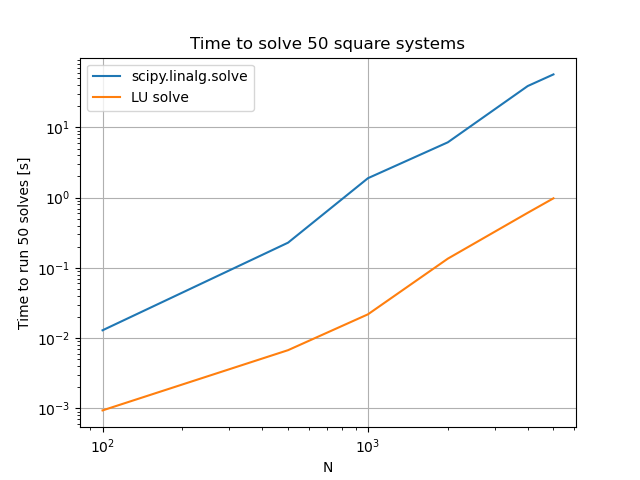
\includegraphics[width=0.5\textwidth]{time.png}
\end{center}

\section{Solving Over Determined Systems}
We wish to find the least squares solution to the system \(A\vec{x} = \vec{b}\), where \(A\) is non square and the system is overdetermined. One approach is to solve the normal equation, \begin{align*}
    A^TA\vec{x} = A^T\vec{b}.
\end{align*} Another approach is to take the QR factorization of \(A\), \(A=QR\), then multiplying by \(Q^T\) we have \begin{align*}
    Q^TQR\vec{x} = Q^T\vec{b}.
\end{align*} Since \(Q\) is orthogonal, this becomes \begin{align*}
    R\vec{x} = Q^T\vec{b},
\end{align*} where the fact that \(R\) is upper triangular may make this faster to solve than the normal equation.

Both techniques for the least squares solution were implemented. Using an error defined as \begin{align*}
    e = |A\vec{x}-b|_2,
\end{align*} the QR algorithm generally achieves a lower error than solving the normal equation. For example, a set of random matrices generated with the code provided yields \(e_{normal} = 0.73, e_{QR} = 0.62\).

As the smallest entry of \(\vec{d}\) is increased and \(A\) becomes increasingly poorly conditioned, the numerical error increases.


{\small \lstinputlisting[language=Python]{lab13_code.py}}

\end{document}
